\documentclass[a4paper,11pt]{report}
\usepackage[T1]{fontenc}
\usepackage[utf8]{inputenc}
\usepackage{lmodern}
\usepackage{hyperref}
\usepackage{graphicx}
\usepackage[english]{babel}

% title and subtitle
\title{\Huge \textbf{Unified Heteregeneous Networking Middleware Project Report}  \\ 
\huge \vspace{5mm} Fall 2015 }
% Author
\author{\textsc{Jincheng Li}}
\hypersetup{
  urlcolor=blue
}

\begin{document}

% \frontmatter
\maketitle

% Auto-generated table of contents, list of figures and list of tables %
\tableofcontents
% \mainmatter

% NEW CHAPTER! %
\chapter{Introduction}
Devices with Internet access today are becoming increasingly mobile. The Heterogeneous Networking Middleware project provides a mechanism for devices to seamlessly handle network mobility, and make intelligent decisions about how and when to use different networks across multiple network interfaces. \\
The project started in 2012 in the IRT lab and went through significant development from 2012 to 2013. After a period of inactivity, it was restarted in Spring 2015 and continued until now (Fall 2015). \\
The prototype for this project started with a demo on Linux and is currently shifting to Android. Some work was done last semester to port the Linux implementation to Android, while this semester we took a different approach and re-implemented some of the necessary functionalities within the Android Java Frameork. \\
In this report, I will cover existing work before I started contributing to the project, research done on Android framework's networking stack, and efforts toward implementing the middleware in Android.

\chapter{Existing Work}
Prior to me being involved in the project, a lot of work has been done on the research on heterogeneous networks and Linux prototype implementation. Porting to Android started in Spring 2015. Here we briefly describe the various network protocols used in the project, and the Linux prototype implementation.

\section{Protocols}
There are three major protocols involved in the construction of the middleware: HIP, MIP, and MIH. HIP and MIP are two mobility protocols that achieve the same goal: ensuring continuous TCP connection in the presence of IP mobility. MIH is part of the IEEE 802.21 standard, providing an informational service that enables seamless handovers between heterogeneous layer-2 network technologies.

\subsection{IP Mobility}
We first introduce the idea of IP mobility. The internet was originally designed with the assumption that an IP address uniquely identifies a host. With multi-homing introduced and the proliferation of mobile internet devices which constantly move between different networks, this is no longer true. Currently, when an internet device switches between different network interfaces, consequently changing its IP address, the TCP (or any other transport protocol) connection in use will break because TCP identifies end-points with IP addresses. Given this, it is desirable to devise a mechanism that maintains the TCP connection when a device changes its IP address. \\
In both HIP and MIP, this is done through maintaining a unique identifier for a device even when the it changes its IP address. The details of how the identifier is defined and maintained varies for different protocols, but the idea stays the same.

\subsection{HIP}
\textbf{Description:} The Host Identity Protocol's approach to IP mobility introduces a Host Identity (HI) namespace based on a public key security infrastructure. Each host generates its own public key and uses the hash of that key as its identifier (or HIT - Host Identity Tag). This identifier encapsulates the host's varying IP address, and remains the same regardless of what new IP address the host obtains. TCP sockets are bound to HITs and therefore the connection does not break even if IP adderss changes. Using public keys has the added advantage of security - the host can conveniently prove its identity with a private-key signature. \\
HIP uses a 4-way handshake process to establish connection between two hosts. In its most general form, assuming both hosts are mobile (and their IP addresses may change), a mobile host initiating the connection talks to the rendevzvous server (RVS) in order to reach the other host. The RVS is responsible for keeping track of IP addresses and HITs of communicating hosts. Then the 4-way handshake process follows, which authenticates the two hosts, negotiates security parameters (through Diffie-Hellman exchange), and establishes ESP security associations (IPSec). The two hosts subsequently communicates through ESP payloads. When the IP address of a mobile host changes, HIP will initiate an update process to inform the other host (and RVS) of the change, so that the mapping from HITs to IP addresses can be updated and subsequent communcation sent to the new IP address. \\
\textbf{Implementation:} We are continuing to use the HIP for Linux implementation available at \url{http://infrahip.hiit.fi/}. It has experimental Android support and is being actively maintained.

\subsection{MIP}
\textbf{Description:} Mobile IP \\
\textbf{Implementation:} We are not using MIP because there does not seem to be any actively-maintained implementations of MIP available. 

\subsection{MIH}
\textbf{Description:} Media-Independent Handover \\
\textbf{Implementation:} 

\section{Linux Implementation}

\chapter{Android Networking Stack}
In order to understand how Android performs intelligent network switching and the functionalities it provides similar to MIH, a fair amount of time was spent this semester researching the architecture of Android's networking stack. The idea is that once we understand the internal structure of Android's networking stack by looking at the source code, we can modify the source code to incorporate functionalities of our middleware into Android. We were able to map out mostly the architecture of Android's network-related classes. Here we present the details of our findings. \\
Note that although there is some similar content in the Spring 2015 student report, the Android OS version studied there is 4.4 KitKat, whereas this document concerns 6.0 Marshmallow. Android introduced some intelligent network-switching functionality in between these two versions, and therefore there can be significant discrepancies between the network infrastructure of the two versions.
\section{Android Architecture}
We first introduce the architecture of the Android platform. Broadly speaking, Android consists of five layers: Linux kernel, HAL, Android runtime + native libraries, Android Framework, and user applications. These five layers are laid out in the following diagram: % elaborate...

% android architecture diagram here
\begin{center}
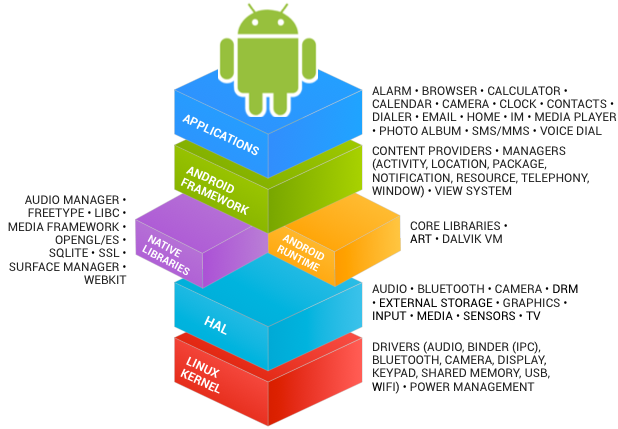
\includegraphics[scale=0.7]{figures/android_framework_details.png}
\end{center}

At the bottom of the Android software stack is the Linux kernel, which provides a level of abstraction between the device hardware and the upper layers of Android. The kernel provides typical low-level system services such as process, memory management, and also includes essential device drivers for hardware such as cellular and WiFi NICs. \\
The hardware abstraction layer (HAL) defines a standard interface for hardware vendors to implement and allows Android to be agnostic about lower-level driver implementations. We don't discuss HAL at any more length here as it is not vital for our purposes. \\
Next comes the Android runtime (i.e. Davlik VM) and native libraries, which are implemented in C/C++. The Dalvik VM is a virtual machine developed by Google to run Java applications on the Linux kernel. It is specifically designed for mobile devices and optimized for memory usage. The libraries at this layer include a subset of standard Java core libraries, and Android libraries including opengl, database (sqlite), webkit, etc. \\
Layered on top of the runtime and libraries is the Android Framework. This framework is implemented entirely in Java, and provides applications with an API that can be used to interact with system services, including UI, telephony, location, etc. This part of Android is what most of the research effort on Android this semester focused on. The Android demo also directly modifies Android Framework's source code to integrate our middleware functionalities into the system. \\
Finally on the top level are applications that interact directly with the user. These include native applications (web browser, settings, email) provided by Google and applications developed by third-party developers.

\section{General Networking}
The following classes deal with network connectivity for all types of networks (cellular, WiFi, or ethernet). This is done through an abstraction called NetworkAgent that encapsulates different types of networks into a common interface, as is explained in more detail later in this section.

\subsection{ConnectivityManager}
Location: \verb|frameworks/base/core/java/android/net/|\\
In general, classes with a ``Manager'' suffix are singleton classes exposed as part of the Android API for applications. They serve as the interface between application developers and the Android framework. Methods in these classes do not usually contain intricate program logic, but simply call some other system service class (e.g. methods in ConnectivityManager call corresponding methods in ConnectivtyService) which actually implements the required functionality. \\
In the case of ConnectivityManager, it is reponsible for answering queries about the state of network connectivity, and for notifying applications about network connectivity changes. Additionally, it allows applications to request or select certain networks for their data traffic. This last feature is most relevant to our research, as it provides an entry point for applications to specify the characteristics of the network they prefer. The implementation of this feature is essentially a simplified version of the middleware's policy engine. An application can choose a policy for its network traffic, and Android will match the network that scores the highest according to that policy to this application. \\
The method invoked for applications to request certain networks is \verb|requestNetwork|, which takes as its input a \verb|NetworkRequest|, and a \verb|NetworkCallback|. As its name suggests, the \verb|NetworkCallback| is invoked once the network is switched to one that satisfies the request. The key component of a \verb|NetworkRequest| is a \verb|NetworkCapabilities| object, representing the capabilities of a network. This is elaborated more in the following subsection.

\subsection{NetworkCapabilities}
\verb|NetworkCapabilities| is the class currently used by Android to record information about a generic network. It contains a number of bit-mask fields indicating whether a network has a certain capability, and also a couple of numeric field such as bandwidth. Specifically, the class records the following capabilities about a network:
\begin{enumerate}
\item services supported: \verb|MMS|, \verb|SUPL|, \verb|DUN|, \verb|FOTA|, \verb|IMS|, \verb|CBS|, \verb|WIFI_P2P|, \verb|IA|, \verb|RCS|, \verb|XCAP|, \verb|EIMS|
\item status: \verb|INTERNET|, \verb|NOT_RESTRICTED|, \verb|TRUSTED|, \verb|VALIDATED|
\item charateristics: \verb|NOT_METERED|, \verb|NOT_VPN|, \verb|CAPTIVE_PORTAL|
\item transport type: \verb|CELLULAR|, \verb|WIFI|, \verb|ETHERNET|, \verb|BLUETOOTH|, \verb|VPN|
\item bandwidth: \verb|LinkUpBandwidth|, \verb|LinkDownBandwidth|
\end{enumerate}
Note that for bandwidth, the numbers are currently an expected value instead of a measured statistic. \\
From the list above, we can see that for the most part the capabilities are binary. As such, the ``scoring'' function used by Android on \verb|NetworkCapabilities| is also straightforward: it simply filters out networks that do not satisfy certain capabilities (i.e. there is no score at this stage, it is only a binary filter). We will describe later how this works with another scoring mechanism that together decide which network is best suited to a \verb|NetworkRequest|.

\subsection{ConnectivityService}
\verb|ConnectivityService| provides implementations of many methods in \verb|ConnectivityManager|. We discuss some of these methods relevant to our research below:
\begin{enumerate}
\item requestNetwork
\item rematchNetworkAndRequests
\end{enumerate}

\subsection{NetworkAgent and NetworkAgentInfo}
NetworkAgent is used by ConnectivityService to keep track of 

\section{WiFi Networks}

\subsection{WifiManager}
The WifiManager class is exposed as part of Android's application API. It provides methods for applications to manage all aspects of WiFi connectivity.

\subsection{WifiService}

\subsection{WifiStateMachine}

\subsection{WifiAutoJoinController}

\section{Cellular Networks}
\subsection{TelephonyManager}
\subsection{DataConnection}

\chapter{Implementation in Android}

\section{Working with the Android Framework}
This section describes the necessary steps to set up and work with the Android framework. Most of this information can also be found on the Android Open-Source Project (AOSP: \url{https://source.android.com/source}) site. This guide documents the specific steps I went through, and any problems I encountered in the process.

\subsection{Environment Setup}

\subsubsection{Requirements}
Developing AOSP typically requires a 64-bit Linux or Mac OS system. I'm using 64-bit Linux Mint 17. As such, the following documentation applies to Linux only (note that Ubuntu should behave the same way as Linux Mint). For more reference on Mac OS, please refer to the AOSP site. Also note that 150 GB of free disk space is recommended for a single build.

\subsubsection{Establishing Build Environment}
Please see the page on AOSP (\url{https://source.android.com/source/initializing.html}) for reference on properly setting up dependencies for the build environment. These are simply some \verb|apt-get| commands and configurations. Note that at the end of the page there is a section called ``Optimizing a build environment'', which enables ccache to speed up recompilation. In my experience this was very helpful for saving compilation time. \\

\subsubsection{Downloading Android Source}
To download the Android source, you first need to have the \verb|repo| tool installed. This can be done with:
\begin{verbatim}
$ sudo curl https://storage.googleapis.com/git-repo-downloads/repo 
  > /usr/local/bin/repo
$ sudo chmod a+x /usr/local/bin/repo
\end{verbatim}
Next, create an empty directory to hold your working files:
\begin{verbatim}
$ mkdir ~/android
\end{verbatim}
Run \verb|repo init| to bring down the latest version of the \verb|repo| tool, and also supply it with a URL for the manifest, which specifies where the various repositories included in the Android source will be placed within your working directory.
\begin{verbatim}
$ repo init -u 
  https://android.googlesource.com/platform/manifest
\end{verbatim}
Note that this defaults to the \verb|master| branch, which is the one I developed on. At the time of writing, the Android version for the \verb|master| branch is 6.0 Marshmallow. It is also possible to download a different version of Android using a different manifest file. \\
Once the initialization is complete, run
\begin{verbatim}
$ repo sync
\end{verbatim}
to pull down the Android source tree. This should take anywhere between a couple hours to a day depending on your connection bandwidth. I believe it took approximately two hours with Columbia's public WiFi network. It is okay to interrupt the process. Running \verb|repo sync| again later will pick up from where the download was left off.

\subsection{Building and Running}
There are two ways to build/run the source code: with an emulator, or with a physical device. The emulator is a bit slow and lacks support for WiFi networks. It runs inside a QEMU hypervisor and has an emulated cellular connection. For physical devices, the only devices that AOSP currently supports are Nexus devices. Any other device requires a build configuration that's not directly available in the provided \verb|lunch| menu. You can find some useful information about non-Nexus device configurations on the CyanogenMod wiki (\url{https://wiki.cyanogenmod.org/w/Main_Page}).
\subsubsection{Building}
First, initialize the build environment by sourcing the \verb|envsetup.sh| script. Inside \verb|~/android| (where Android source is downloaded to), run
\begin{verbatim}
$ source build/envsetup.sh
\end{verbatim}
This includes several utility functions into the shell, which are necessary for building the source. Note that only \verb|bash| is compatible with these functions, so make sure you are not using another shell. \\
Next, choose a target to build with \verb|lunch|. You can see a list of possible targets by running \verb|lunch| without an argument, or you can choose a target directly with, for instance,
\begin{verbatim}
$ lunch aosp-arm_eng
\end{verbatim}
which builds the emulator with all debugging enabled. \\
Finally, build everything with \verb|make|. It is recommended to build using the \verb|-jN| argument, which parallelizes the build process. The fastest builds are ususally made with number of tasks N between 1 and 2 times the number of hardware threads on the computer. For example, for a computer with 8 cores, the fastest builds are between \verb|make -j8| and \verb|make -j16|.
\subsubsection{Running}
To run an emulator build, simply run \verb|emulator| in the terminal. To run a device-specific build, you can flash it onto the device with \verb|fastboot|. In order to flash a device, connect the device to your computer, and run
\begin{verbatim}
$ adb reboot bootloader
\end{verbatim}
which reboots the device into fastboot mode, and then run
\begin{verbatim}
$ fastboot flashall -w
\end{verbatim}
which flashes the system image onto the device.\\
For more information on running builds and choosing the appropriate build configuration for a device, see \url{https://source.android.com/source/running.html}.

\subsection{Developing}

\subsubsection{Repository Management}
As previously mentioned, \verb|repo| is used to manage development of the Android project. Development of a new topic branch typically starts with
\begin{verbatim}
$ repo start <BRANCH_NAME> [<PROJECT_LIST>]
\end{verbatim}
This will create a branch with the given name in each of the \verb|git| projects included in \verb|<PROJECT_LIST>|. Afterwards, simply proceed as usual to each of the projects, make some changes, and commit them separately with \verb|git|. You can use \verb|repo status [<PROJECT_LIST>]| to check the status of each of the projects. \\
Unfortunately there is no easy way to upload your changes to a remote repository. The \verb|repo| tool is designed to let you upload your changes to the Google source code server and submit them for review, eventually merging into the \verb|master| branch. However, since we are working on an experimental project with limited time, this is not a desired method. For now I have saved my changes as \verb|patch| files and uploaded them to Github (\url{https://github.com/jchli/hetnet-report}). You can apply them with \verb|git am|. 

\subsubsection{Testing}
Once changes are made, run the \verb|make -jN| command to build Android, and then either use the emulator or flash a physcial device to test the operating system. I have personally been testing the system on emulator only because there was no Nexus device with more than one type of network. \\
There are two debugging tools that I found helpful with testing: \verb|adb logcat| and \verb|telnet|, which are detailed below.
\begin{enumerate}
\item When browsing Android code you will notice lots of logging lines. These system debug messages are stored in a buffer and can all be viewed and filtered with \verb|adb logcat|. The syntax for doing so is
\begin{verbatim}
$ adb logcat [filter-options]
\end{verbatim}
Every debug message has a tag and a priority. The tag is used to indicate which part of the system the message came from. This is frequently the name of the class where the message was collected from (e.g. ConnectivityService). There are a number of priorities for debugging messages: V (verbose), D (debug), I (info), W, (warning), E (error), F (fatal), S (silent). You can use a combination of tags and priorities to filter debug messages. For example, the following command
\begin{verbatim}
$ adb logcat ConnectivityService:* *:S
\end{verbatim}
prints all debug messages with the ConnectivityService tag, and silences all other messages.
\item The second useful debugging tool works with the emulator only. Each emulator instance provides a control console that you can connect to, to issue commands to that instance. If you are only running one emulator instance (as is usually the case), you can use \verb|telnet localhost 5554| to connect to the console. \\
The console provides several useful functionalities, among which is geo location provider emulation. Inside the console, you can issue commands such as \verb|geo fix <longitude> <latitude>| to send a fixed GPS location to the emulator. This can be particularly useful for our purposes since our policy vector consists of the location parameter.
\end{enumerate}

\section{Android Demo Implementation}
This section talks about implementation of the demo in Android. 

\end{document}
